\chapter{Sequenzdiagramme}

\section{Rezept erstellen und veröffentlichen }
\begin{figure}[H]
	\centering
	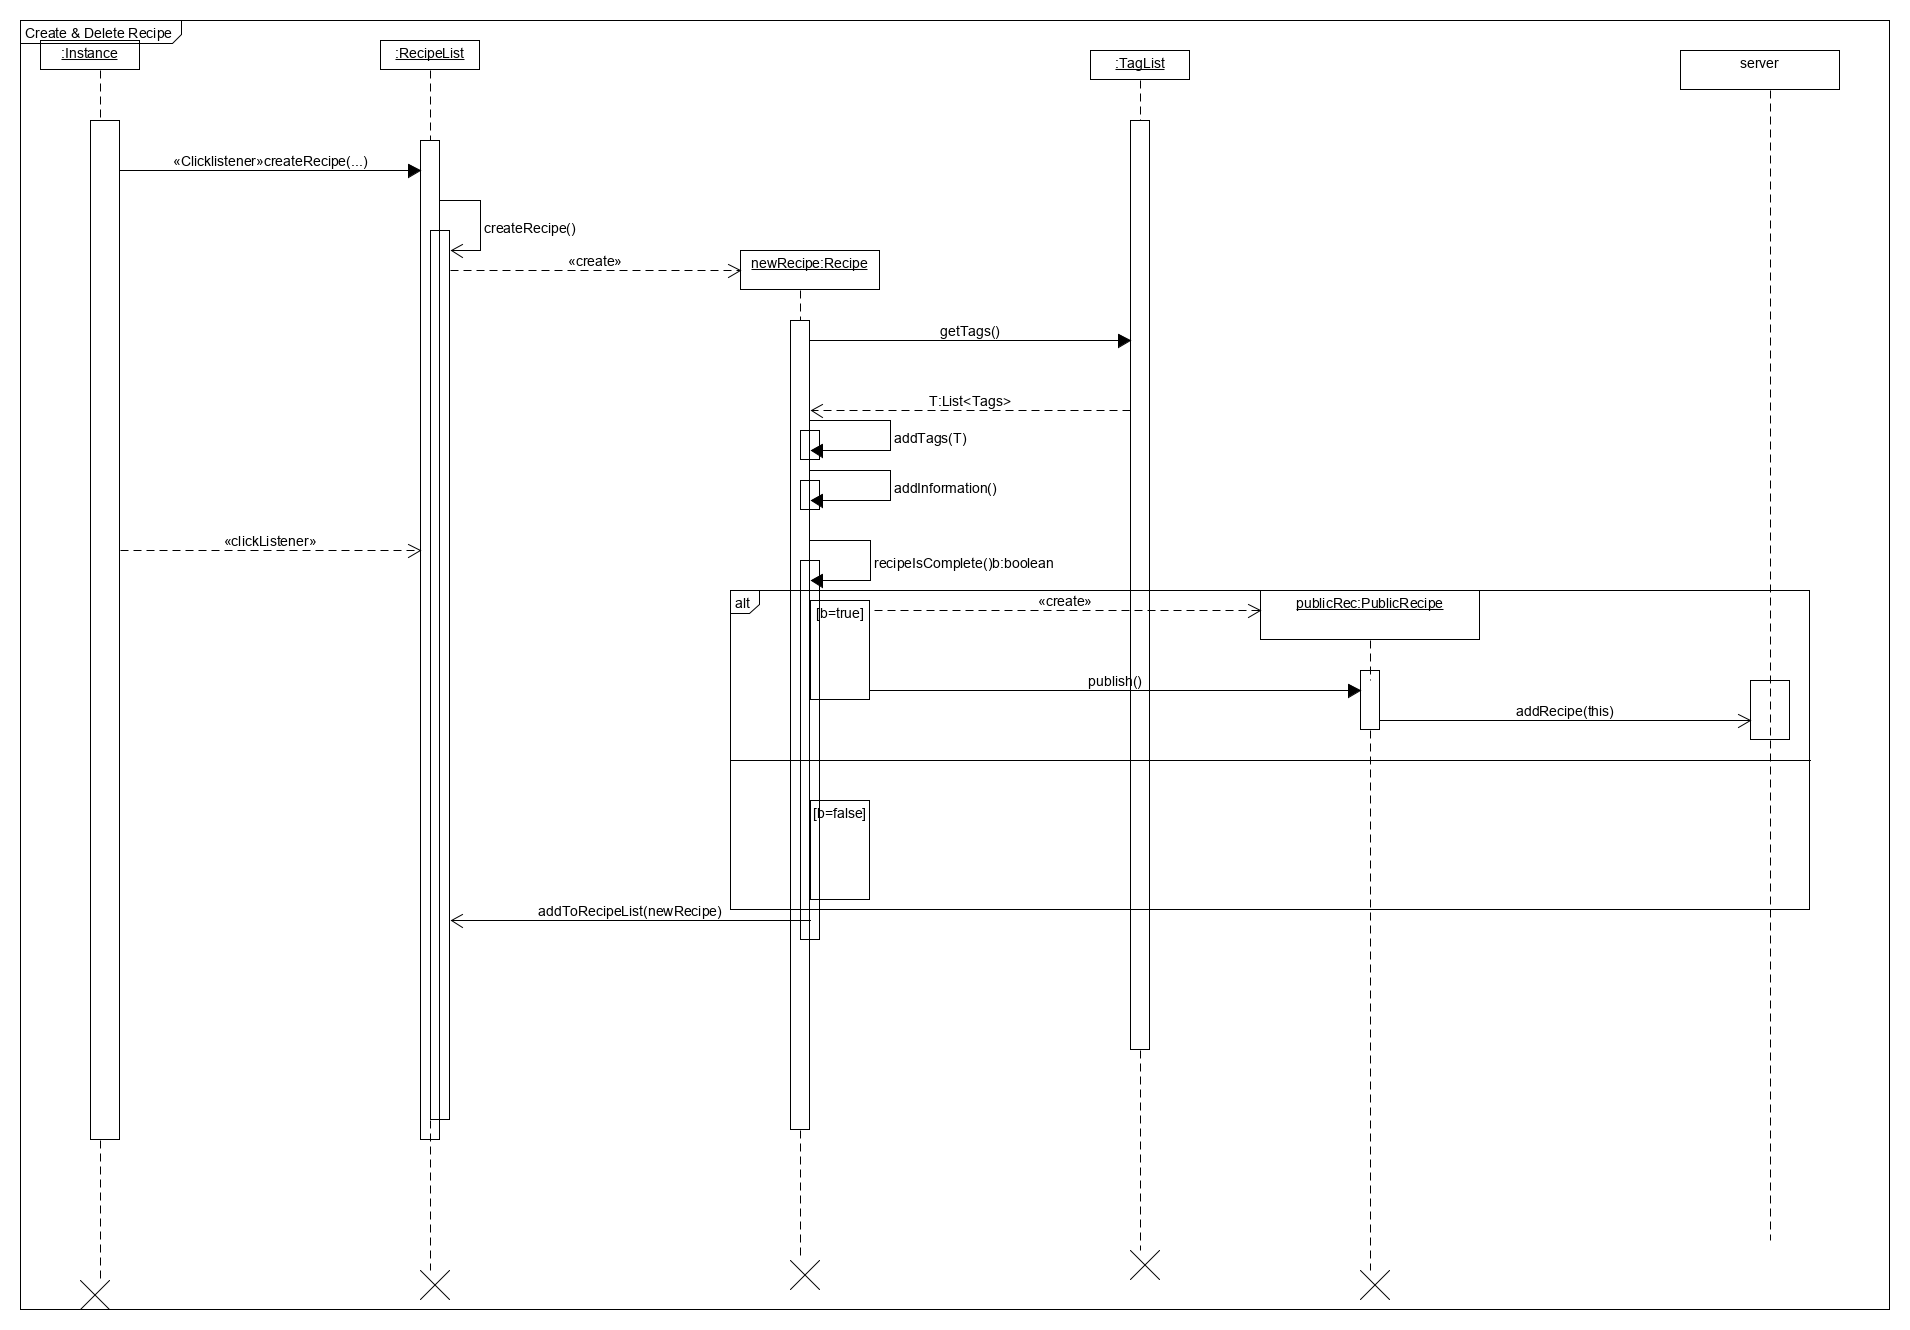
\includegraphics[width=\textwidth]{pics/dynamicDiagram/CreatePublishRecipeSequenceD.png}%
	\caption{Create \& Publish Recipe Sequence Diagram}%
	\label{diagram}%
\end{figure}

Der Nutzer befindet sich in der App, genauer in seiner privaten Rezeptliste. Daraufhin wählt er "Rezept erstellen" aus und wird in das dafür vorgesehene Fragment weitergeleitet. Dort wird ein neues privates Rezept erstellt, mit Tags und Eingaben gefüllt und gespeichert. Da der Nutzer dieses auch veröffentlichen möchte, wird das Rezept auf Vollständigkeit geprüft und in ein öffentliches Rezept konvertiert. Nachdem es veröffentlicht wurde, kehrt der Nutzer zu seiner Rezeptliste Zurück, wo das Rezept nun hinzugefügt wurde. 
  
  
  
  
  \section{Lazy Loading }
  \begin{figure}[H]
  	\centering
  	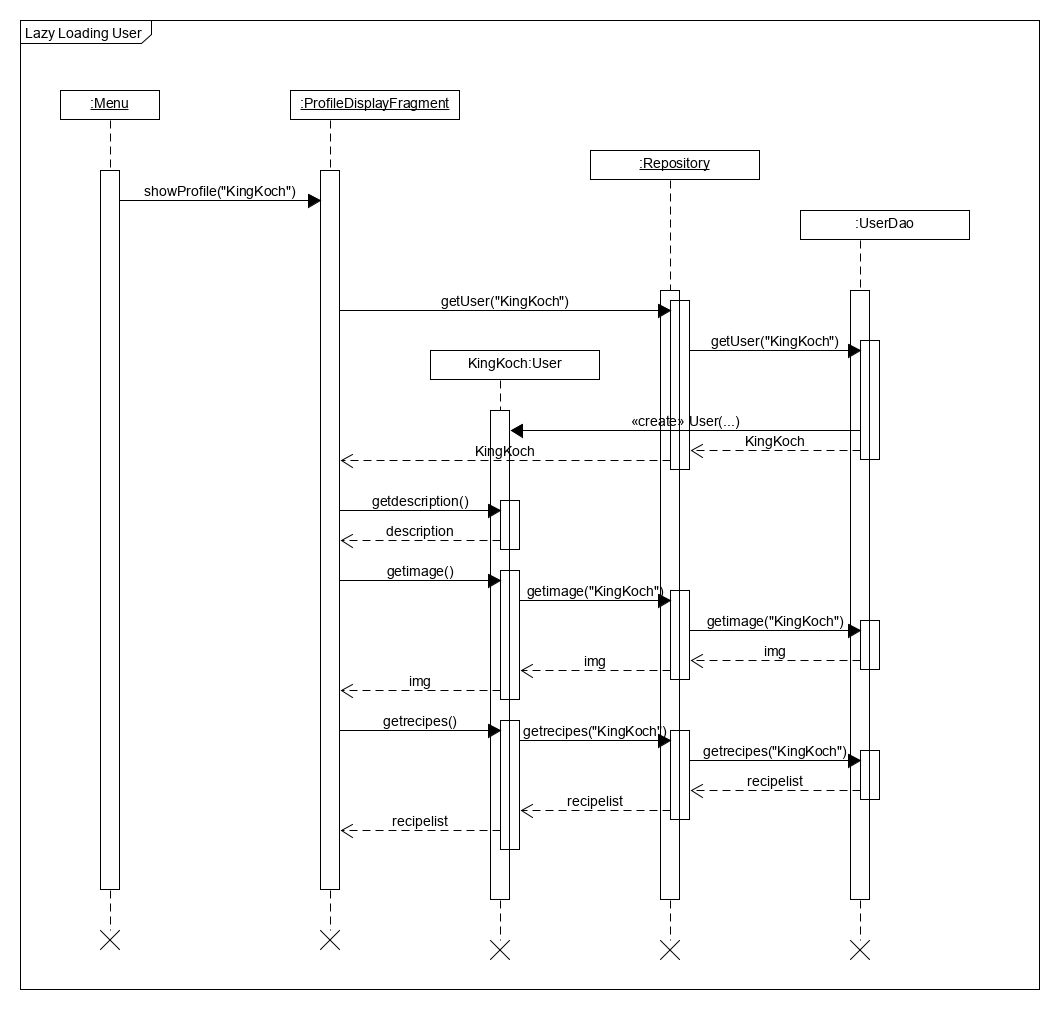
\includegraphics[width=\textwidth]{pics/dynamicDiagram/LazyLoadingUser_SequenzeD.png}%
  	\caption{Lazy Loading User}%
  	\label{diagram}%
  \end{figure}
  
Wenn ein Profil eines Benutzers angezeigt werden soll, wird ein User Objekt erstellt. Es werden manche Attribute direkt initialisiert, wie zum Beispiel die Zubereitung (getdescription()), aber zum Beispiel das Bild und die Kommentare werden erst vom Server geladen, wenn diese auch benutzt werden. Somit wird bei dem getimage() Aufruf erst aus dem Repository die Daten geladen und diese dann zurückgegeben.
  \section{Favorit hinzufügen und entfernen}
\begin{figure}[H]
	\centering
	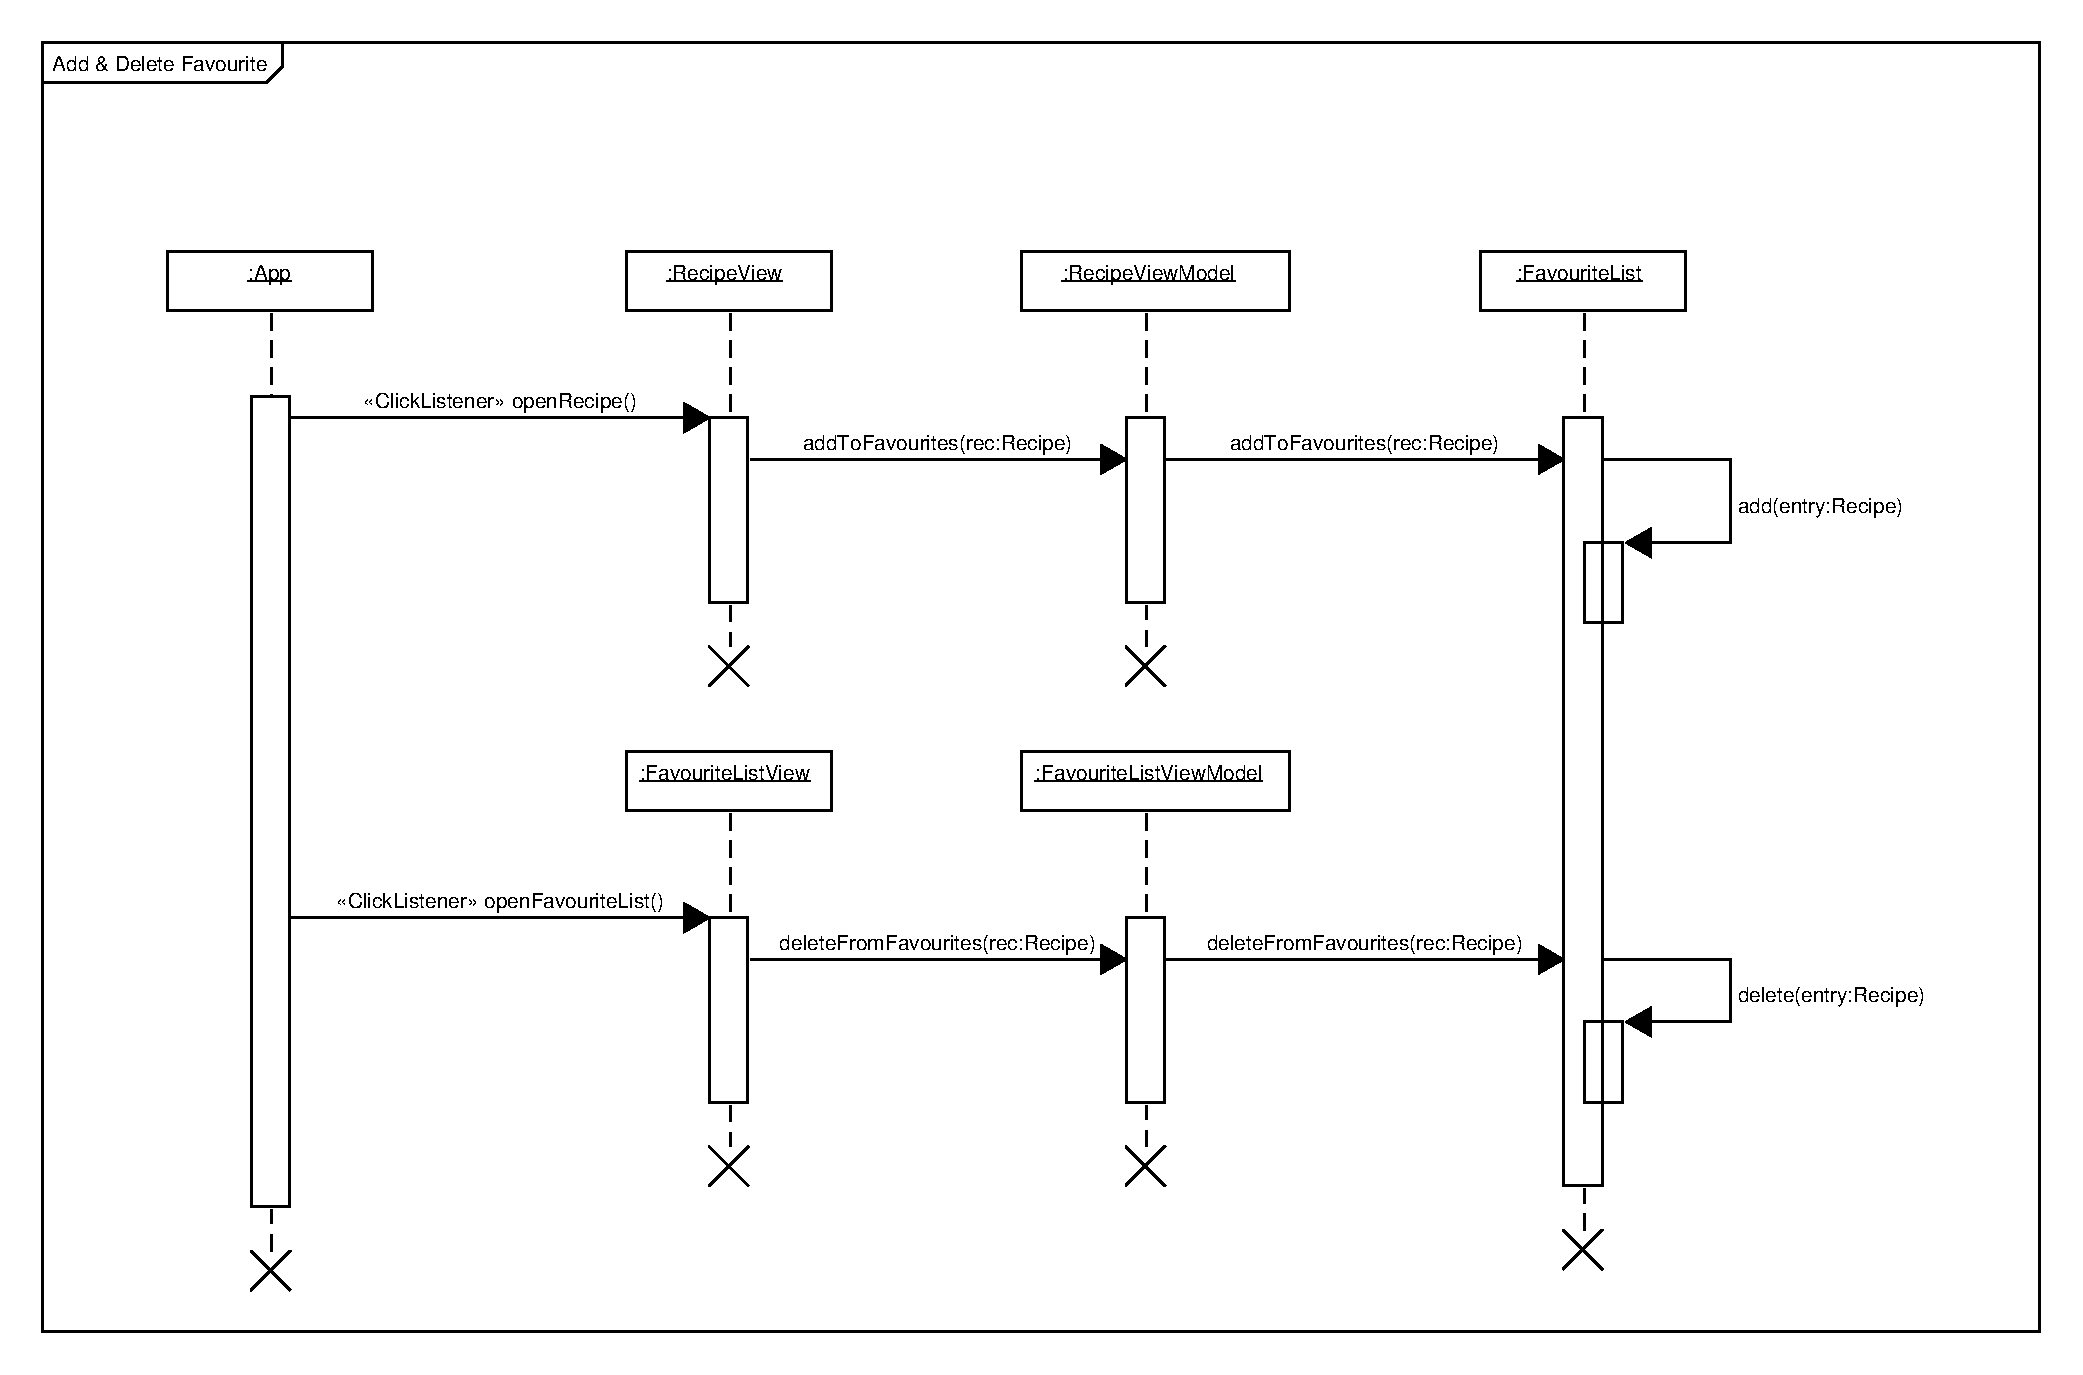
\includegraphics[width=\textwidth]{pics/dynamicDiagram/AddFav_DeleteFav_Recipe_SequenceD.pdf}%
	\caption{Favorit hinzufügen und entfernen}%
	\label{diagram}%
\end{figure}

Der Nutzer hat in der Suche ein Rezept gefunden und öffnet dieses. In der Rezept Anzeige wählt er aus, dass Rezept zu seinen Favoriten hinzuzufügen. Über das ViewModel kann die Information verarbeitet werden und der Favoritenliste des Nutzers wird jenes Rezept hinzugefügt. 
Der Nutzer entscheidet sich dafür ein Rezept aus seiner Favoritenliste zu entfernen. Er wählt bei dem Rezept den Entfernen Button, woraufhin über das ViewModel das Rezept aus der Favoritenliste des Nutzers entfernt wird.

  

  